Para a criação de um tarefa de aprendizado que seja capaz de verificar a autenticidade de assinaturas de indivíduos, é necessário primeiramente a existência de um conjunto de dados de imagens que possuam exemplos de assinaturas forjadas e genuínas. Para isto, utilizou-se o conjunto de imagens disponibilizado pela Competição de Verificação de Assinaturas de 2009 (SigComp2009, do inglês \emph{Signature Verification Competition}) realizado na Conferência Internacional em Análise e Reconhecimento de Documentos (ICDAR, do inglês \emph{International Conference on Document Analysis and Recognition}).

O conjunto disponibilizado pela SigComp2009 é composto por dois tipos de dados da assinaturas, os dados \emph{offline} e os dados \emph{online}. Nos dados \emph{offline}, é considerado apenas os aspectos estáticos da assinatura, ou seja, uma imagem obtida após o processo da assinatura ter sido concluído. Os dados do tipo \emph{online}, por sua vez, contêm informações dinâmicas da assinatura, que consiste em um arquivo de texto com informações capturadas em vários pontos durante o processo da assinatura, sendo estas as coordenadas $x$ e $y$ da ponta da caneta, a pressão exercida sobre a caneta, o ângulo de azimute,

O conjunto disponibilizado pela SigComp2009 pode ser dividido em dois subconjuntos, nos quais um deles possui apenas assinaturas \emph{offline} e \emph{online}, nas quais as assinaturas \emph{offline} s

\begin{figure}[h!]
\centering
\caption{Uma amostra das assinaturas \emph{offline} e \emph{online}. Font: \cite{icdar2009}}
\label{fig:sample-signature}
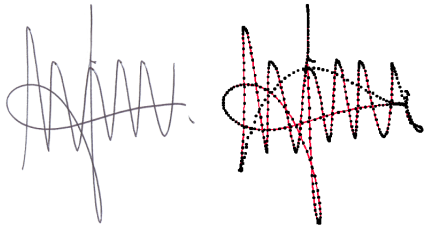
\includegraphics[width=0.6\textwidth]{imgs/sample-signature}
\end{figure}


% Conjuntos de treino e validação disponibilizados pela competição (NISDCC e NFI)
% Assinaturas online e offline
% Como foram feitas as assinaturas forjadas
% A quantidade de indivíduos no dataset
% A quantidade de assinaturas por indivíduo
